\documentclass{article}

\usepackage{xcolor}

\usepackage{tikz}
\usetikzlibrary{mindmap,trees,shadows}
\usetikzlibrary{arrows}

\usepackage{color}
\definecolor{blue1}{RGB}{0,102,189}
\definecolor{blue2}{RGB}{98,160,214}
\definecolor{my_orange}{RGB}{243,98,33}

\usepackage{amsmath}
\usepackage{amssymb} % mathbb


\begin{document}

\thispagestyle{empty}


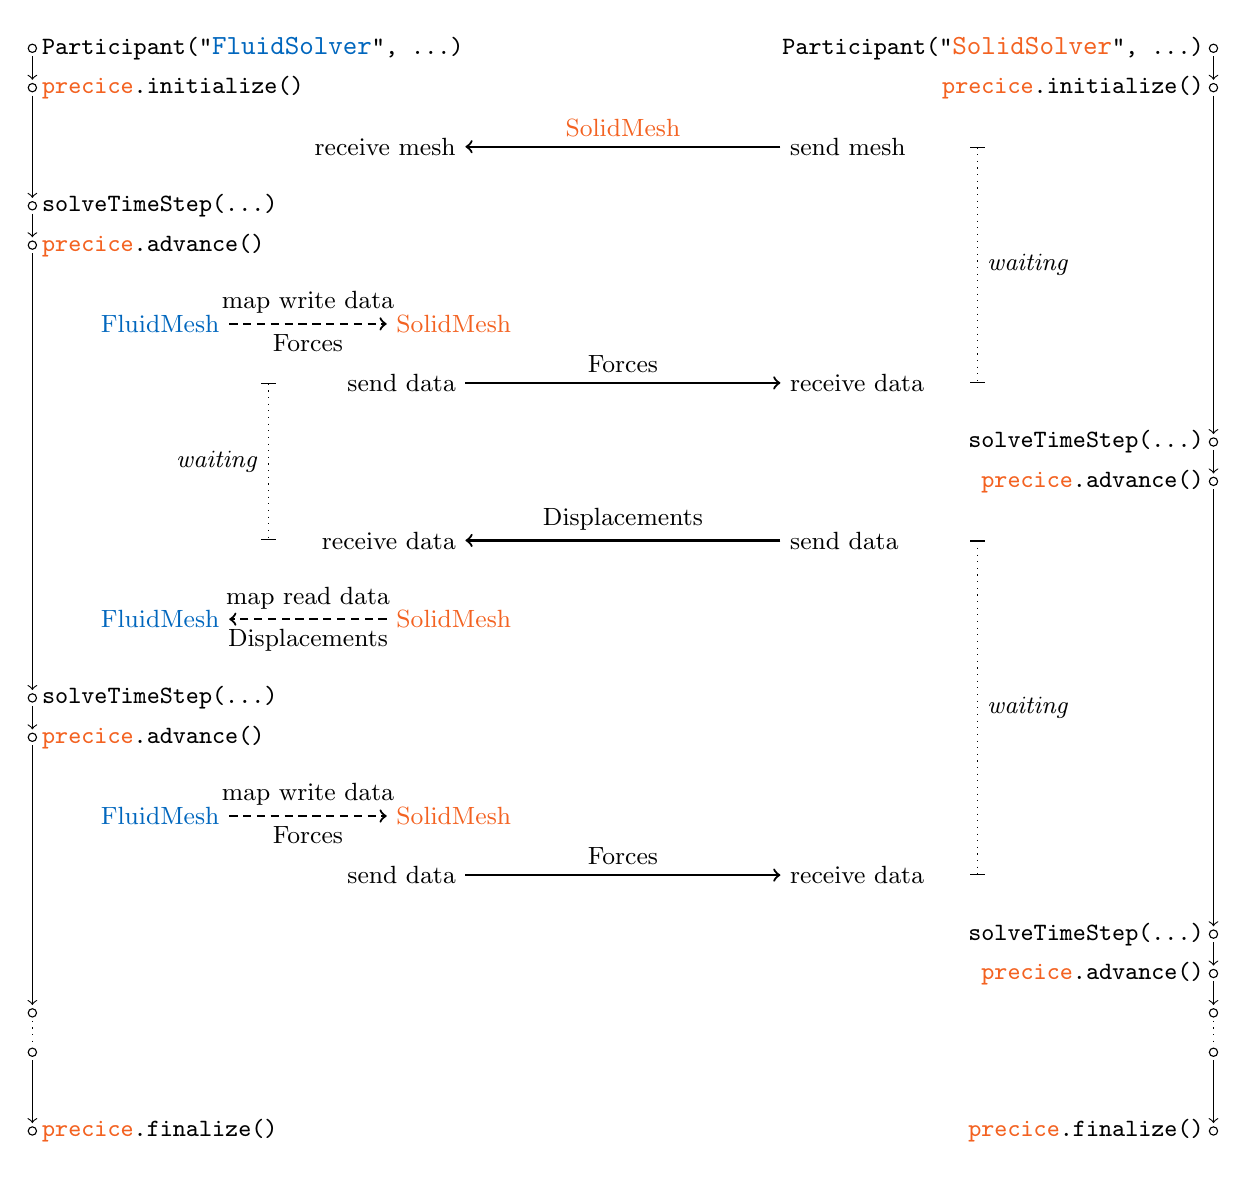
\begin{tikzpicture}

 \coordinate (FE) at (0,0.25);
 \coordinate (SE) at (15,0.25);
 \coordinate (F0) at (0,14);
 \coordinate (S0) at (15,14);
 \draw (F0) circle (1.5pt);
 \draw (FE) circle (1.5pt);
 \draw (S0) circle (1.5pt);
 \draw (SE) circle (1.5pt);
 
 \node[right] at (F0) {\small \texttt{Participant("{\normalsize\color{blue1}{FluidSolver}}", \ldots)}};
 \node[left] at (S0) {\small \texttt{Participant("{\normalsize\color{my_orange}{SolidSolver}}", \ldots)}};

\coordinate (F2) at (0,13.5);
\coordinate (S2) at (15,13.5);
\node[right] at (F2) {\small \texttt{{\color{my_orange}{precice}}.initialize()}};
\node[left] at (S2) {\small \texttt{{\color{my_orange}{precice}}.initialize()}};
\draw (F2) circle (1.5pt);
\draw (S2) circle (1.5pt);

\coordinate (F_mesh) at (5.5,12.75);
\node[left] at (F_mesh) {\small receive mesh};
\coordinate (S_mesh) at (9.5,12.75);
\node[right] at (S_mesh) {\small send mesh};
\draw[->,thick] (S_mesh) -- (F_mesh) node[midway,above] {\small \color{my_orange} SolidMesh};


\coordinate (F3) at (0,12);
\coordinate (S3) at (15,9);
\node[right] at (F3) {\small \texttt{solveTimeStep(\ldots)}};
\node[left] at (S3) {\small \texttt{solveTimeStep(\ldots)}};
\draw (F3) circle (1.5pt);
\draw (S3) circle (1.5pt);

\coordinate (F4) at (0,11.5);
\coordinate (S4) at (15,8.5);
\node[right] at (F4) {\small \texttt{{\color{my_orange}{precice}}.advance()}};
\node[left] at (S4) {\small \texttt{{\color{my_orange}{precice}}.advance()}};
\draw (F4) circle (1.5pt);
\draw (S4) circle (1.5pt);

\coordinate (F_map1) at (2.5,10.5);
\node[left] at (F_map1) {\small \color{blue1} FluidMesh};
\coordinate (F_map2) at (4.5,10.5);
\node[right] at (F_map2) {\small \color{my_orange} SolidMesh};
\draw[->, thick, densely dashed] (F_map1) -- (F_map2) node[midway,above] {\small map write data} node[midway,below] {\small Forces};

\draw[|-|, dotted] (12,12.75) to node[midway,right] {\small \textit{waiting}} (12,9.75);


\coordinate (F_com1) at (5.5,9.75);
\node[left] at (F_com1) {\small send data};
\coordinate (S_com1) at (9.5,9.75);
\node[right] at (S_com1) {\small receive data};
\draw[->,thick,out=0,in=180] (F_com1) to node[midway,above] {\small  Forces} (S_com1);


\coordinate (F_com2) at (5.5,7.75);
\node[left] at (F_com2) {\small receive data};
\coordinate (S_com2) at (9.5,7.75);
\node[right] at (S_com2) {\small send data};
\draw[->,thick, out=180,in=0] (S_com2) to node[midway,above] {\small   Displacements} (F_com2);

\draw[|-|, dotted] (3,9.75) to node[midway,left] {\small \textit{waiting}} (3,7.75);


%\node[right] at (9.5,7.75) {\small accelerate data};

\coordinate (F_map3) at (2.5,6.75);
\node[left] at (F_map3) {\small \color{blue1} FluidMesh};
\coordinate (F_map4) at (4.5,6.75);
\node[right] at (F_map4) {\small \color{my_orange} SolidMesh};
\draw[->, thick, densely dashed] (F_map4) -- (F_map3) node[midway,above] {\small map read data} node[midway,below] {\small Displacements};

\coordinate (F5) at (0,5.75);
\coordinate (S5) at (15,2.75);
\node[right] at (F5) {\small  \texttt{solveTimeStep(\ldots)}};
\node[left] at (S5) {\small \texttt{solveTimeStep(\ldots)}};
\draw (F5) circle (1.5pt);
\draw (S5) circle (1.5pt);

\coordinate (F6) at (0,5.25);
\coordinate (S6) at (15,2.25);
\node[right] at (F6) {\small \texttt{{\color{my_orange}{precice}}.advance()}};
\node[left] at (S6) {\small \texttt{{\color{my_orange}{precice}}.advance()}};
\draw (F6) circle (1.5pt);
\draw (S6) circle (1.5pt);

\coordinate (F_map5) at (2.5,4.25);
\node[left] at (F_map5) {\small \color{blue1} FluidMesh};
\coordinate (F_map6) at (4.5,4.25);
\node[right] at (F_map6) {\small \color{my_orange} SolidMesh};
\draw[->, thick, densely dashed] (F_map5) -- (F_map6) node[midway,above] {\small map write data} node[midway,below] {\small Forces};

\coordinate (F_com3) at (5.5,3.5);
\node[left] at (F_com3) {\small send data};
\coordinate (S_com3) at (9.5,3.5);
\node[right] at (S_com3) {\small receive data};
\draw[->,thick,out=0,in=180] (F_com3) to node[midway,above] {\small   Forces} (S_com3);

\draw[|-|, dotted] (12,7.75) to node[midway,right] {\small \textit{waiting}} (12,3.5);

\coordinate (F7) at (0,1.75);
\coordinate (S7) at (15,1.75);
\draw (F7) circle (1.5pt);
\draw (S7) circle (1.5pt);

\coordinate (F8) at (0,1.25);
\coordinate (S8) at (15,1.25);
\draw (F8) circle (1.5pt);
\draw (S8) circle (1.5pt);

\node[right] at (FE) {\small \texttt{{\color{my_orange}{precice}}.finalize()}};
\node[left] at (SE) {\small \texttt{{\color{my_orange}{precice}}.finalize()}};

\draw [->, shorten <=.1cm, shorten >=.1cm] (F0) to (F2);
\draw [->, shorten <=.1cm, shorten >=.1cm] (F2) to (F3);
\draw [->, shorten <=.1cm, shorten >=.1cm] (F3) to (F4);
\draw [->, shorten <=.1cm, shorten >=.1cm] (F4) to (F5);
\draw [->, shorten <=.1cm, shorten >=.1cm] (F5) to (F6);
\draw [->, shorten <=.1cm, shorten >=.1cm] (F6) to (F7);
\draw [dotted, shorten <=.1cm, shorten >=.1cm] (F7) to (F8);
\draw [->, shorten <=.1cm, shorten >=.1cm] (F8) to (FE);
\draw [->, shorten <=.1cm, shorten >=.1cm] (S0) to (S2);
\draw [->, shorten <=.1cm, shorten >=.1cm] (S2) to (S3);
\draw [->, shorten <=.1cm, shorten >=.1cm] (S3) to (S4);
\draw [->, shorten <=.1cm, shorten >=.1cm] (S4) to (S5);
\draw [->, shorten <=.1cm, shorten >=.1cm] (S5) to (S6);
\draw [->, shorten <=.1cm, shorten >=.1cm] (S6) to (S7);
\draw [dotted, shorten <=.1cm, shorten >=.1cm] (S7) to (S8);
\draw [->, shorten <=.1cm, shorten >=.1cm] (S8) to (SE);
\end{tikzpicture}

\end{document}
